% Created by tikzDevice version 0.10.1 on 2018-01-01 00:15:22
% !TEX encoding = UTF-8 Unicode
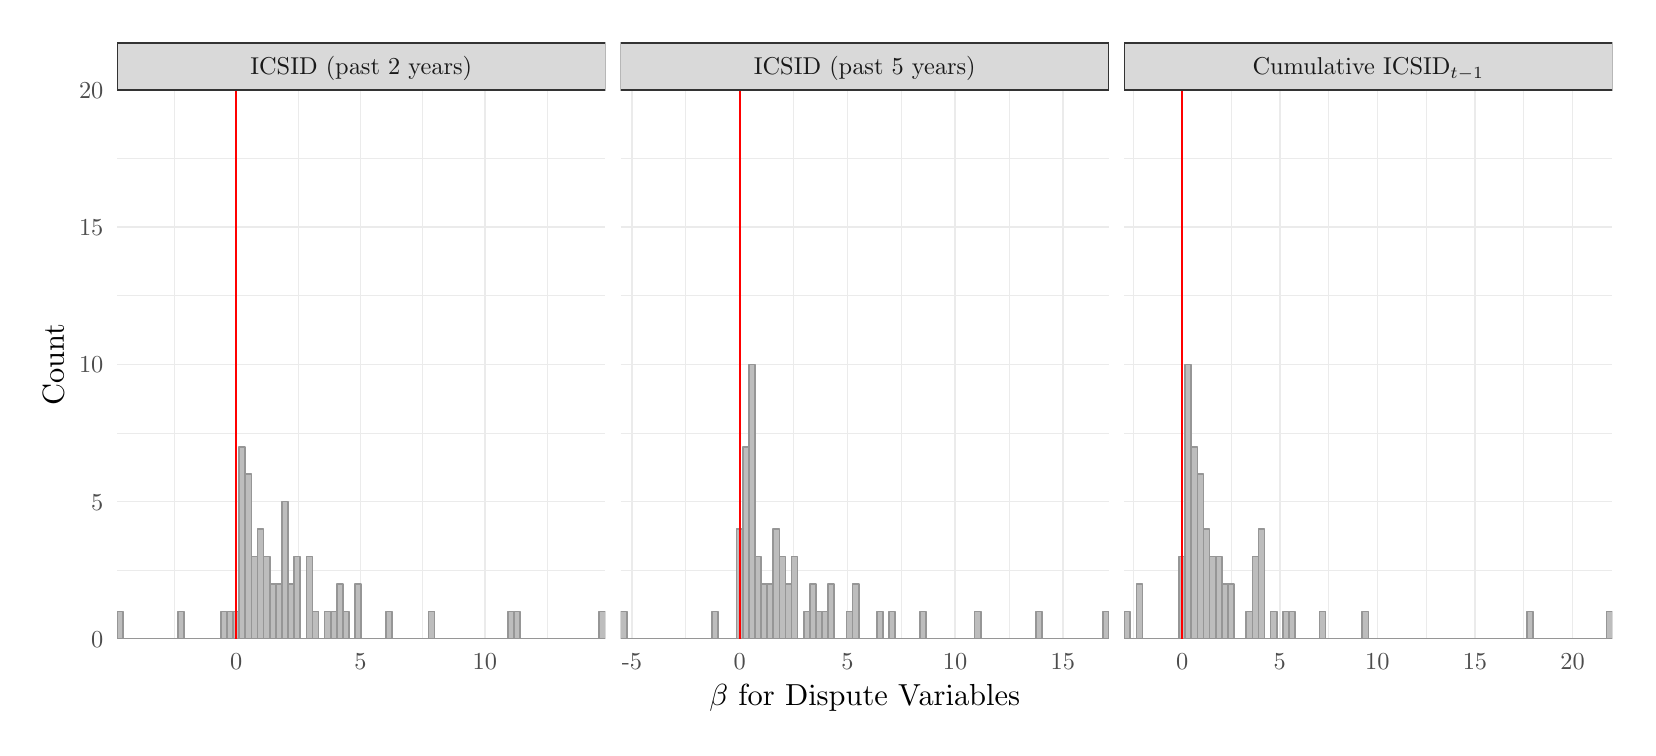
\begin{tikzpicture}[x=1pt,y=1pt]
\definecolor{fillColor}{RGB}{255,255,255}
\path[use as bounding box,fill=fillColor,fill opacity=0.00] (0,0) rectangle (578.16,252.94);
\begin{scope}
\path[clip] (  0.00,  0.00) rectangle (578.16,252.94);
\definecolor{drawColor}{RGB}{255,255,255}
\definecolor{fillColor}{RGB}{255,255,255}

\path[draw=drawColor,line width= 0.6pt,line join=round,line cap=round,fill=fillColor] (  0.00, -0.00) rectangle (578.16,252.94);
\end{scope}
\begin{scope}
\path[clip] ( 32.32, 32.09) rectangle (208.77,230.38);
\definecolor{fillColor}{RGB}{255,255,255}

\path[fill=fillColor] ( 32.32, 32.09) rectangle (208.77,230.38);
\definecolor{drawColor}{gray}{0.92}

\path[draw=drawColor,line width= 0.3pt,line join=round] ( 32.32, 56.87) --
	(208.77, 56.87);

\path[draw=drawColor,line width= 0.3pt,line join=round] ( 32.32,106.45) --
	(208.77,106.45);

\path[draw=drawColor,line width= 0.3pt,line join=round] ( 32.32,156.02) --
	(208.77,156.02);

\path[draw=drawColor,line width= 0.3pt,line join=round] ( 32.32,205.60) --
	(208.77,205.60);

\path[draw=drawColor,line width= 0.3pt,line join=round] ( 52.87, 32.09) --
	( 52.87,230.38);

\path[draw=drawColor,line width= 0.3pt,line join=round] ( 97.79, 32.09) --
	( 97.79,230.38);

\path[draw=drawColor,line width= 0.3pt,line join=round] (142.71, 32.09) --
	(142.71,230.38);

\path[draw=drawColor,line width= 0.3pt,line join=round] (187.63, 32.09) --
	(187.63,230.38);

\path[draw=drawColor,line width= 0.6pt,line join=round] ( 32.32, 32.09) --
	(208.77, 32.09);

\path[draw=drawColor,line width= 0.6pt,line join=round] ( 32.32, 81.66) --
	(208.77, 81.66);

\path[draw=drawColor,line width= 0.6pt,line join=round] ( 32.32,131.24) --
	(208.77,131.24);

\path[draw=drawColor,line width= 0.6pt,line join=round] ( 32.32,180.81) --
	(208.77,180.81);

\path[draw=drawColor,line width= 0.6pt,line join=round] ( 32.32,230.38) --
	(208.77,230.38);

\path[draw=drawColor,line width= 0.6pt,line join=round] ( 75.33, 32.09) --
	( 75.33,230.38);

\path[draw=drawColor,line width= 0.6pt,line join=round] (120.25, 32.09) --
	(120.25,230.38);

\path[draw=drawColor,line width= 0.6pt,line join=round] (165.17, 32.09) --
	(165.17,230.38);
\definecolor{drawColor}{gray}{0.59}
\definecolor{fillColor}{gray}{0.74}

\path[draw=drawColor,line width= 0.6pt,line join=round,fill=fillColor] ( 32.32, 32.09) rectangle ( 34.53, 42.00);

\path[draw=drawColor,line width= 0.6pt,line join=round,fill=fillColor] ( 34.53, 32.09) rectangle ( 36.73, 32.09);

\path[draw=drawColor,line width= 0.6pt,line join=round,fill=fillColor] ( 36.73, 32.09) rectangle ( 38.94, 32.09);

\path[draw=drawColor,line width= 0.6pt,line join=round,fill=fillColor] ( 38.94, 32.09) rectangle ( 41.15, 32.09);

\path[draw=drawColor,line width= 0.6pt,line join=round,fill=fillColor] ( 41.15, 32.09) rectangle ( 43.35, 32.09);

\path[draw=drawColor,line width= 0.6pt,line join=round,fill=fillColor] ( 43.35, 32.09) rectangle ( 45.56, 32.09);

\path[draw=drawColor,line width= 0.6pt,line join=round,fill=fillColor] ( 45.56, 32.09) rectangle ( 47.76, 32.09);

\path[draw=drawColor,line width= 0.6pt,line join=round,fill=fillColor] ( 47.76, 32.09) rectangle ( 49.97, 32.09);

\path[draw=drawColor,line width= 0.6pt,line join=round,fill=fillColor] ( 49.97, 32.09) rectangle ( 52.17, 32.09);

\path[draw=drawColor,line width= 0.6pt,line join=round,fill=fillColor] ( 52.17, 32.09) rectangle ( 54.38, 32.09);

\path[draw=drawColor,line width= 0.6pt,line join=round,fill=fillColor] ( 54.38, 32.09) rectangle ( 56.59, 42.00);

\path[draw=drawColor,line width= 0.6pt,line join=round,fill=fillColor] ( 56.59, 32.09) rectangle ( 58.79, 32.09);

\path[draw=drawColor,line width= 0.6pt,line join=round,fill=fillColor] ( 58.79, 32.09) rectangle ( 61.00, 32.09);

\path[draw=drawColor,line width= 0.6pt,line join=round,fill=fillColor] ( 61.00, 32.09) rectangle ( 63.20, 32.09);

\path[draw=drawColor,line width= 0.6pt,line join=round,fill=fillColor] ( 63.20, 32.09) rectangle ( 65.41, 32.09);

\path[draw=drawColor,line width= 0.6pt,line join=round,fill=fillColor] ( 65.41, 32.09) rectangle ( 67.61, 32.09);

\path[draw=drawColor,line width= 0.6pt,line join=round,fill=fillColor] ( 67.61, 32.09) rectangle ( 69.82, 32.09);

\path[draw=drawColor,line width= 0.6pt,line join=round,fill=fillColor] ( 69.82, 32.09) rectangle ( 72.02, 42.00);

\path[draw=drawColor,line width= 0.6pt,line join=round,fill=fillColor] ( 72.02, 32.09) rectangle ( 74.23, 42.00);

\path[draw=drawColor,line width= 0.6pt,line join=round,fill=fillColor] ( 74.23, 32.09) rectangle ( 76.44, 42.00);

\path[draw=drawColor,line width= 0.6pt,line join=round,fill=fillColor] ( 76.44, 32.09) rectangle ( 78.64,101.49);

\path[draw=drawColor,line width= 0.6pt,line join=round,fill=fillColor] ( 78.64, 32.09) rectangle ( 80.85, 91.58);

\path[draw=drawColor,line width= 0.6pt,line join=round,fill=fillColor] ( 80.85, 32.09) rectangle ( 83.05, 61.83);

\path[draw=drawColor,line width= 0.6pt,line join=round,fill=fillColor] ( 83.05, 32.09) rectangle ( 85.26, 71.75);

\path[draw=drawColor,line width= 0.6pt,line join=round,fill=fillColor] ( 85.26, 32.09) rectangle ( 87.46, 61.83);

\path[draw=drawColor,line width= 0.6pt,line join=round,fill=fillColor] ( 87.46, 32.09) rectangle ( 89.67, 51.92);

\path[draw=drawColor,line width= 0.6pt,line join=round,fill=fillColor] ( 89.67, 32.09) rectangle ( 91.87, 51.92);

\path[draw=drawColor,line width= 0.6pt,line join=round,fill=fillColor] ( 91.87, 32.09) rectangle ( 94.08, 81.66);

\path[draw=drawColor,line width= 0.6pt,line join=round,fill=fillColor] ( 94.08, 32.09) rectangle ( 96.29, 51.92);

\path[draw=drawColor,line width= 0.6pt,line join=round,fill=fillColor] ( 96.29, 32.09) rectangle ( 98.49, 61.83);

\path[draw=drawColor,line width= 0.6pt,line join=round,fill=fillColor] ( 98.49, 32.09) rectangle (100.70, 32.09);

\path[draw=drawColor,line width= 0.6pt,line join=round,fill=fillColor] (100.70, 32.09) rectangle (102.90, 61.83);

\path[draw=drawColor,line width= 0.6pt,line join=round,fill=fillColor] (102.90, 32.09) rectangle (105.11, 42.00);

\path[draw=drawColor,line width= 0.6pt,line join=round,fill=fillColor] (105.11, 32.09) rectangle (107.31, 32.09);

\path[draw=drawColor,line width= 0.6pt,line join=round,fill=fillColor] (107.31, 32.09) rectangle (109.52, 42.00);

\path[draw=drawColor,line width= 0.6pt,line join=round,fill=fillColor] (109.52, 32.09) rectangle (111.72, 42.00);

\path[draw=drawColor,line width= 0.6pt,line join=round,fill=fillColor] (111.72, 32.09) rectangle (113.93, 51.92);

\path[draw=drawColor,line width= 0.6pt,line join=round,fill=fillColor] (113.93, 32.09) rectangle (116.14, 42.00);

\path[draw=drawColor,line width= 0.6pt,line join=round,fill=fillColor] (116.14, 32.09) rectangle (118.34, 32.09);

\path[draw=drawColor,line width= 0.6pt,line join=round,fill=fillColor] (118.34, 32.09) rectangle (120.55, 51.92);

\path[draw=drawColor,line width= 0.6pt,line join=round,fill=fillColor] (120.55, 32.09) rectangle (122.75, 32.09);

\path[draw=drawColor,line width= 0.6pt,line join=round,fill=fillColor] (122.75, 32.09) rectangle (124.96, 32.09);

\path[draw=drawColor,line width= 0.6pt,line join=round,fill=fillColor] (124.96, 32.09) rectangle (127.16, 32.09);

\path[draw=drawColor,line width= 0.6pt,line join=round,fill=fillColor] (127.16, 32.09) rectangle (129.37, 32.09);

\path[draw=drawColor,line width= 0.6pt,line join=round,fill=fillColor] (129.37, 32.09) rectangle (131.57, 42.00);

\path[draw=drawColor,line width= 0.6pt,line join=round,fill=fillColor] (131.57, 32.09) rectangle (133.78, 32.09);

\path[draw=drawColor,line width= 0.6pt,line join=round,fill=fillColor] (133.78, 32.09) rectangle (135.99, 32.09);

\path[draw=drawColor,line width= 0.6pt,line join=round,fill=fillColor] (135.99, 32.09) rectangle (138.19, 32.09);

\path[draw=drawColor,line width= 0.6pt,line join=round,fill=fillColor] (138.19, 32.09) rectangle (140.40, 32.09);

\path[draw=drawColor,line width= 0.6pt,line join=round,fill=fillColor] (140.40, 32.09) rectangle (142.60, 32.09);

\path[draw=drawColor,line width= 0.6pt,line join=round,fill=fillColor] (142.60, 32.09) rectangle (144.81, 32.09);

\path[draw=drawColor,line width= 0.6pt,line join=round,fill=fillColor] (144.81, 32.09) rectangle (147.01, 42.00);

\path[draw=drawColor,line width= 0.6pt,line join=round,fill=fillColor] (147.01, 32.09) rectangle (149.22, 32.09);

\path[draw=drawColor,line width= 0.6pt,line join=round,fill=fillColor] (149.22, 32.09) rectangle (151.42, 32.09);

\path[draw=drawColor,line width= 0.6pt,line join=round,fill=fillColor] (151.42, 32.09) rectangle (153.63, 32.09);

\path[draw=drawColor,line width= 0.6pt,line join=round,fill=fillColor] (153.63, 32.09) rectangle (155.84, 32.09);

\path[draw=drawColor,line width= 0.6pt,line join=round,fill=fillColor] (155.84, 32.09) rectangle (158.04, 32.09);

\path[draw=drawColor,line width= 0.6pt,line join=round,fill=fillColor] (158.04, 32.09) rectangle (160.25, 32.09);

\path[draw=drawColor,line width= 0.6pt,line join=round,fill=fillColor] (160.25, 32.09) rectangle (162.45, 32.09);

\path[draw=drawColor,line width= 0.6pt,line join=round,fill=fillColor] (162.45, 32.09) rectangle (164.66, 32.09);

\path[draw=drawColor,line width= 0.6pt,line join=round,fill=fillColor] (164.66, 32.09) rectangle (166.86, 32.09);

\path[draw=drawColor,line width= 0.6pt,line join=round,fill=fillColor] (166.86, 32.09) rectangle (169.07, 32.09);

\path[draw=drawColor,line width= 0.6pt,line join=round,fill=fillColor] (169.07, 32.09) rectangle (171.27, 32.09);

\path[draw=drawColor,line width= 0.6pt,line join=round,fill=fillColor] (171.27, 32.09) rectangle (173.48, 32.09);

\path[draw=drawColor,line width= 0.6pt,line join=round,fill=fillColor] (173.48, 32.09) rectangle (175.69, 42.00);

\path[draw=drawColor,line width= 0.6pt,line join=round,fill=fillColor] (175.69, 32.09) rectangle (177.89, 42.00);

\path[draw=drawColor,line width= 0.6pt,line join=round,fill=fillColor] (177.89, 32.09) rectangle (180.10, 32.09);

\path[draw=drawColor,line width= 0.6pt,line join=round,fill=fillColor] (180.10, 32.09) rectangle (182.30, 32.09);

\path[draw=drawColor,line width= 0.6pt,line join=round,fill=fillColor] (182.30, 32.09) rectangle (184.51, 32.09);

\path[draw=drawColor,line width= 0.6pt,line join=round,fill=fillColor] (184.51, 32.09) rectangle (186.71, 32.09);

\path[draw=drawColor,line width= 0.6pt,line join=round,fill=fillColor] (186.71, 32.09) rectangle (188.92, 32.09);

\path[draw=drawColor,line width= 0.6pt,line join=round,fill=fillColor] (188.92, 32.09) rectangle (191.12, 32.09);

\path[draw=drawColor,line width= 0.6pt,line join=round,fill=fillColor] (191.12, 32.09) rectangle (193.33, 32.09);

\path[draw=drawColor,line width= 0.6pt,line join=round,fill=fillColor] (193.33, 32.09) rectangle (195.54, 32.09);

\path[draw=drawColor,line width= 0.6pt,line join=round,fill=fillColor] (195.54, 32.09) rectangle (197.74, 32.09);

\path[draw=drawColor,line width= 0.6pt,line join=round,fill=fillColor] (197.74, 32.09) rectangle (199.95, 32.09);

\path[draw=drawColor,line width= 0.6pt,line join=round,fill=fillColor] (199.95, 32.09) rectangle (202.15, 32.09);

\path[draw=drawColor,line width= 0.6pt,line join=round,fill=fillColor] (202.15, 32.09) rectangle (204.36, 32.09);

\path[draw=drawColor,line width= 0.6pt,line join=round,fill=fillColor] (204.36, 32.09) rectangle (206.56, 32.09);

\path[draw=drawColor,line width= 0.6pt,line join=round,fill=fillColor] (206.56, 32.09) rectangle (208.77, 42.00);
\definecolor{drawColor}{RGB}{255,0,0}

\path[draw=drawColor,line width= 0.6pt,line join=round] ( 75.33, 32.09) -- ( 75.33,230.38);
\end{scope}
\begin{scope}
\path[clip] (214.27, 32.09) rectangle (390.71,230.38);
\definecolor{fillColor}{RGB}{255,255,255}

\path[fill=fillColor] (214.27, 32.09) rectangle (390.71,230.38);
\definecolor{drawColor}{gray}{0.92}

\path[draw=drawColor,line width= 0.3pt,line join=round] (214.27, 56.87) --
	(390.71, 56.87);

\path[draw=drawColor,line width= 0.3pt,line join=round] (214.27,106.45) --
	(390.71,106.45);

\path[draw=drawColor,line width= 0.3pt,line join=round] (214.27,156.02) --
	(390.71,156.02);

\path[draw=drawColor,line width= 0.3pt,line join=round] (214.27,205.60) --
	(390.71,205.60);

\path[draw=drawColor,line width= 0.3pt,line join=round] (237.82, 32.09) --
	(237.82,230.38);

\path[draw=drawColor,line width= 0.3pt,line join=round] (276.74, 32.09) --
	(276.74,230.38);

\path[draw=drawColor,line width= 0.3pt,line join=round] (315.65, 32.09) --
	(315.65,230.38);

\path[draw=drawColor,line width= 0.3pt,line join=round] (354.57, 32.09) --
	(354.57,230.38);

\path[draw=drawColor,line width= 0.6pt,line join=round] (214.27, 32.09) --
	(390.71, 32.09);

\path[draw=drawColor,line width= 0.6pt,line join=round] (214.27, 81.66) --
	(390.71, 81.66);

\path[draw=drawColor,line width= 0.6pt,line join=round] (214.27,131.24) --
	(390.71,131.24);

\path[draw=drawColor,line width= 0.6pt,line join=round] (214.27,180.81) --
	(390.71,180.81);

\path[draw=drawColor,line width= 0.6pt,line join=round] (214.27,230.38) --
	(390.71,230.38);

\path[draw=drawColor,line width= 0.6pt,line join=round] (218.36, 32.09) --
	(218.36,230.38);

\path[draw=drawColor,line width= 0.6pt,line join=round] (257.28, 32.09) --
	(257.28,230.38);

\path[draw=drawColor,line width= 0.6pt,line join=round] (296.19, 32.09) --
	(296.19,230.38);

\path[draw=drawColor,line width= 0.6pt,line join=round] (335.11, 32.09) --
	(335.11,230.38);

\path[draw=drawColor,line width= 0.6pt,line join=round] (374.03, 32.09) --
	(374.03,230.38);
\definecolor{drawColor}{gray}{0.59}
\definecolor{fillColor}{gray}{0.74}

\path[draw=drawColor,line width= 0.6pt,line join=round,fill=fillColor] (214.27, 32.09) rectangle (216.47, 42.00);

\path[draw=drawColor,line width= 0.6pt,line join=round,fill=fillColor] (216.47, 32.09) rectangle (218.68, 32.09);

\path[draw=drawColor,line width= 0.6pt,line join=round,fill=fillColor] (218.68, 32.09) rectangle (220.89, 32.09);

\path[draw=drawColor,line width= 0.6pt,line join=round,fill=fillColor] (220.89, 32.09) rectangle (223.09, 32.09);

\path[draw=drawColor,line width= 0.6pt,line join=round,fill=fillColor] (223.09, 32.09) rectangle (225.30, 32.09);

\path[draw=drawColor,line width= 0.6pt,line join=round,fill=fillColor] (225.30, 32.09) rectangle (227.50, 32.09);

\path[draw=drawColor,line width= 0.6pt,line join=round,fill=fillColor] (227.50, 32.09) rectangle (229.71, 32.09);

\path[draw=drawColor,line width= 0.6pt,line join=round,fill=fillColor] (229.71, 32.09) rectangle (231.91, 32.09);

\path[draw=drawColor,line width= 0.6pt,line join=round,fill=fillColor] (231.91, 32.09) rectangle (234.12, 32.09);

\path[draw=drawColor,line width= 0.6pt,line join=round,fill=fillColor] (234.12, 32.09) rectangle (236.32, 32.09);

\path[draw=drawColor,line width= 0.6pt,line join=round,fill=fillColor] (236.32, 32.09) rectangle (238.53, 32.09);

\path[draw=drawColor,line width= 0.6pt,line join=round,fill=fillColor] (238.53, 32.09) rectangle (240.74, 32.09);

\path[draw=drawColor,line width= 0.6pt,line join=round,fill=fillColor] (240.74, 32.09) rectangle (242.94, 32.09);

\path[draw=drawColor,line width= 0.6pt,line join=round,fill=fillColor] (242.94, 32.09) rectangle (245.15, 32.09);

\path[draw=drawColor,line width= 0.6pt,line join=round,fill=fillColor] (245.15, 32.09) rectangle (247.35, 32.09);

\path[draw=drawColor,line width= 0.6pt,line join=round,fill=fillColor] (247.35, 32.09) rectangle (249.56, 42.00);

\path[draw=drawColor,line width= 0.6pt,line join=round,fill=fillColor] (249.56, 32.09) rectangle (251.76, 32.09);

\path[draw=drawColor,line width= 0.6pt,line join=round,fill=fillColor] (251.76, 32.09) rectangle (253.97, 32.09);

\path[draw=drawColor,line width= 0.6pt,line join=round,fill=fillColor] (253.97, 32.09) rectangle (256.18, 32.09);

\path[draw=drawColor,line width= 0.6pt,line join=round,fill=fillColor] (256.18, 32.09) rectangle (258.38, 71.75);

\path[draw=drawColor,line width= 0.6pt,line join=round,fill=fillColor] (258.38, 32.09) rectangle (260.59,101.49);

\path[draw=drawColor,line width= 0.6pt,line join=round,fill=fillColor] (260.59, 32.09) rectangle (262.79,131.24);

\path[draw=drawColor,line width= 0.6pt,line join=round,fill=fillColor] (262.79, 32.09) rectangle (265.00, 61.83);

\path[draw=drawColor,line width= 0.6pt,line join=round,fill=fillColor] (265.00, 32.09) rectangle (267.20, 51.92);

\path[draw=drawColor,line width= 0.6pt,line join=round,fill=fillColor] (267.20, 32.09) rectangle (269.41, 51.92);

\path[draw=drawColor,line width= 0.6pt,line join=round,fill=fillColor] (269.41, 32.09) rectangle (271.61, 71.75);

\path[draw=drawColor,line width= 0.6pt,line join=round,fill=fillColor] (271.61, 32.09) rectangle (273.82, 61.83);

\path[draw=drawColor,line width= 0.6pt,line join=round,fill=fillColor] (273.82, 32.09) rectangle (276.03, 51.92);

\path[draw=drawColor,line width= 0.6pt,line join=round,fill=fillColor] (276.03, 32.09) rectangle (278.23, 61.83);

\path[draw=drawColor,line width= 0.6pt,line join=round,fill=fillColor] (278.23, 32.09) rectangle (280.44, 32.09);

\path[draw=drawColor,line width= 0.6pt,line join=round,fill=fillColor] (280.44, 32.09) rectangle (282.64, 42.00);

\path[draw=drawColor,line width= 0.6pt,line join=round,fill=fillColor] (282.64, 32.09) rectangle (284.85, 51.92);

\path[draw=drawColor,line width= 0.6pt,line join=round,fill=fillColor] (284.85, 32.09) rectangle (287.05, 42.00);

\path[draw=drawColor,line width= 0.6pt,line join=round,fill=fillColor] (287.05, 32.09) rectangle (289.26, 42.00);

\path[draw=drawColor,line width= 0.6pt,line join=round,fill=fillColor] (289.26, 32.09) rectangle (291.46, 51.92);

\path[draw=drawColor,line width= 0.6pt,line join=round,fill=fillColor] (291.46, 32.09) rectangle (293.67, 32.09);

\path[draw=drawColor,line width= 0.6pt,line join=round,fill=fillColor] (293.67, 32.09) rectangle (295.88, 32.09);

\path[draw=drawColor,line width= 0.6pt,line join=round,fill=fillColor] (295.88, 32.09) rectangle (298.08, 42.00);

\path[draw=drawColor,line width= 0.6pt,line join=round,fill=fillColor] (298.08, 32.09) rectangle (300.29, 51.92);

\path[draw=drawColor,line width= 0.6pt,line join=round,fill=fillColor] (300.29, 32.09) rectangle (302.49, 32.09);

\path[draw=drawColor,line width= 0.6pt,line join=round,fill=fillColor] (302.49, 32.09) rectangle (304.70, 32.09);

\path[draw=drawColor,line width= 0.6pt,line join=round,fill=fillColor] (304.70, 32.09) rectangle (306.90, 32.09);

\path[draw=drawColor,line width= 0.6pt,line join=round,fill=fillColor] (306.90, 32.09) rectangle (309.11, 42.00);

\path[draw=drawColor,line width= 0.6pt,line join=round,fill=fillColor] (309.11, 32.09) rectangle (311.31, 32.09);

\path[draw=drawColor,line width= 0.6pt,line join=round,fill=fillColor] (311.31, 32.09) rectangle (313.52, 42.00);

\path[draw=drawColor,line width= 0.6pt,line join=round,fill=fillColor] (313.52, 32.09) rectangle (315.73, 32.09);

\path[draw=drawColor,line width= 0.6pt,line join=round,fill=fillColor] (315.73, 32.09) rectangle (317.93, 32.09);

\path[draw=drawColor,line width= 0.6pt,line join=round,fill=fillColor] (317.93, 32.09) rectangle (320.14, 32.09);

\path[draw=drawColor,line width= 0.6pt,line join=round,fill=fillColor] (320.14, 32.09) rectangle (322.34, 32.09);

\path[draw=drawColor,line width= 0.6pt,line join=round,fill=fillColor] (322.34, 32.09) rectangle (324.55, 42.00);

\path[draw=drawColor,line width= 0.6pt,line join=round,fill=fillColor] (324.55, 32.09) rectangle (326.75, 32.09);

\path[draw=drawColor,line width= 0.6pt,line join=round,fill=fillColor] (326.75, 32.09) rectangle (328.96, 32.09);

\path[draw=drawColor,line width= 0.6pt,line join=round,fill=fillColor] (328.96, 32.09) rectangle (331.16, 32.09);

\path[draw=drawColor,line width= 0.6pt,line join=round,fill=fillColor] (331.16, 32.09) rectangle (333.37, 32.09);

\path[draw=drawColor,line width= 0.6pt,line join=round,fill=fillColor] (333.37, 32.09) rectangle (335.58, 32.09);

\path[draw=drawColor,line width= 0.6pt,line join=round,fill=fillColor] (335.58, 32.09) rectangle (337.78, 32.09);

\path[draw=drawColor,line width= 0.6pt,line join=round,fill=fillColor] (337.78, 32.09) rectangle (339.99, 32.09);

\path[draw=drawColor,line width= 0.6pt,line join=round,fill=fillColor] (339.99, 32.09) rectangle (342.19, 32.09);

\path[draw=drawColor,line width= 0.6pt,line join=round,fill=fillColor] (342.19, 32.09) rectangle (344.40, 42.00);

\path[draw=drawColor,line width= 0.6pt,line join=round,fill=fillColor] (344.40, 32.09) rectangle (346.60, 32.09);

\path[draw=drawColor,line width= 0.6pt,line join=round,fill=fillColor] (346.60, 32.09) rectangle (348.81, 32.09);

\path[draw=drawColor,line width= 0.6pt,line join=round,fill=fillColor] (348.81, 32.09) rectangle (351.01, 32.09);

\path[draw=drawColor,line width= 0.6pt,line join=round,fill=fillColor] (351.01, 32.09) rectangle (353.22, 32.09);

\path[draw=drawColor,line width= 0.6pt,line join=round,fill=fillColor] (353.22, 32.09) rectangle (355.43, 32.09);

\path[draw=drawColor,line width= 0.6pt,line join=round,fill=fillColor] (355.43, 32.09) rectangle (357.63, 32.09);

\path[draw=drawColor,line width= 0.6pt,line join=round,fill=fillColor] (357.63, 32.09) rectangle (359.84, 32.09);

\path[draw=drawColor,line width= 0.6pt,line join=round,fill=fillColor] (359.84, 32.09) rectangle (362.04, 32.09);

\path[draw=drawColor,line width= 0.6pt,line join=round,fill=fillColor] (362.04, 32.09) rectangle (364.25, 32.09);

\path[draw=drawColor,line width= 0.6pt,line join=round,fill=fillColor] (364.25, 32.09) rectangle (366.45, 42.00);

\path[draw=drawColor,line width= 0.6pt,line join=round,fill=fillColor] (366.45, 32.09) rectangle (368.66, 32.09);

\path[draw=drawColor,line width= 0.6pt,line join=round,fill=fillColor] (368.66, 32.09) rectangle (370.86, 32.09);

\path[draw=drawColor,line width= 0.6pt,line join=round,fill=fillColor] (370.86, 32.09) rectangle (373.07, 32.09);

\path[draw=drawColor,line width= 0.6pt,line join=round,fill=fillColor] (373.07, 32.09) rectangle (375.28, 32.09);

\path[draw=drawColor,line width= 0.6pt,line join=round,fill=fillColor] (375.28, 32.09) rectangle (377.48, 32.09);

\path[draw=drawColor,line width= 0.6pt,line join=round,fill=fillColor] (377.48, 32.09) rectangle (379.69, 32.09);

\path[draw=drawColor,line width= 0.6pt,line join=round,fill=fillColor] (379.69, 32.09) rectangle (381.89, 32.09);

\path[draw=drawColor,line width= 0.6pt,line join=round,fill=fillColor] (381.89, 32.09) rectangle (384.10, 32.09);

\path[draw=drawColor,line width= 0.6pt,line join=round,fill=fillColor] (384.10, 32.09) rectangle (386.30, 32.09);

\path[draw=drawColor,line width= 0.6pt,line join=round,fill=fillColor] (386.30, 32.09) rectangle (388.51, 32.09);

\path[draw=drawColor,line width= 0.6pt,line join=round,fill=fillColor] (388.51, 32.09) rectangle (390.71, 42.00);
\definecolor{drawColor}{RGB}{255,0,0}

\path[draw=drawColor,line width= 0.6pt,line join=round] (257.28, 32.09) -- (257.28,230.38);
\end{scope}
\begin{scope}
\path[clip] (396.21, 32.09) rectangle (572.66,230.38);
\definecolor{fillColor}{RGB}{255,255,255}

\path[fill=fillColor] (396.21, 32.09) rectangle (572.66,230.38);
\definecolor{drawColor}{gray}{0.92}

\path[draw=drawColor,line width= 0.3pt,line join=round] (396.21, 56.87) --
	(572.66, 56.87);

\path[draw=drawColor,line width= 0.3pt,line join=round] (396.21,106.45) --
	(572.66,106.45);

\path[draw=drawColor,line width= 0.3pt,line join=round] (396.21,156.02) --
	(572.66,156.02);

\path[draw=drawColor,line width= 0.3pt,line join=round] (396.21,205.60) --
	(572.66,205.60);

\path[draw=drawColor,line width= 0.3pt,line join=round] (399.53, 32.09) --
	(399.53,230.38);

\path[draw=drawColor,line width= 0.3pt,line join=round] (434.80, 32.09) --
	(434.80,230.38);

\path[draw=drawColor,line width= 0.3pt,line join=round] (470.07, 32.09) --
	(470.07,230.38);

\path[draw=drawColor,line width= 0.3pt,line join=round] (505.33, 32.09) --
	(505.33,230.38);

\path[draw=drawColor,line width= 0.3pt,line join=round] (540.60, 32.09) --
	(540.60,230.38);

\path[draw=drawColor,line width= 0.6pt,line join=round] (396.21, 32.09) --
	(572.66, 32.09);

\path[draw=drawColor,line width= 0.6pt,line join=round] (396.21, 81.66) --
	(572.66, 81.66);

\path[draw=drawColor,line width= 0.6pt,line join=round] (396.21,131.24) --
	(572.66,131.24);

\path[draw=drawColor,line width= 0.6pt,line join=round] (396.21,180.81) --
	(572.66,180.81);

\path[draw=drawColor,line width= 0.6pt,line join=round] (396.21,230.38) --
	(572.66,230.38);

\path[draw=drawColor,line width= 0.6pt,line join=round] (417.17, 32.09) --
	(417.17,230.38);

\path[draw=drawColor,line width= 0.6pt,line join=round] (452.43, 32.09) --
	(452.43,230.38);

\path[draw=drawColor,line width= 0.6pt,line join=round] (487.70, 32.09) --
	(487.70,230.38);

\path[draw=drawColor,line width= 0.6pt,line join=round] (522.97, 32.09) --
	(522.97,230.38);

\path[draw=drawColor,line width= 0.6pt,line join=round] (558.23, 32.09) --
	(558.23,230.38);
\definecolor{drawColor}{gray}{0.59}
\definecolor{fillColor}{gray}{0.74}

\path[draw=drawColor,line width= 0.6pt,line join=round,fill=fillColor] (396.21, 32.09) rectangle (398.42, 42.00);

\path[draw=drawColor,line width= 0.6pt,line join=round,fill=fillColor] (398.42, 32.09) rectangle (400.63, 32.09);

\path[draw=drawColor,line width= 0.6pt,line join=round,fill=fillColor] (400.63, 32.09) rectangle (402.83, 51.92);

\path[draw=drawColor,line width= 0.6pt,line join=round,fill=fillColor] (402.83, 32.09) rectangle (405.04, 32.09);

\path[draw=drawColor,line width= 0.6pt,line join=round,fill=fillColor] (405.04, 32.09) rectangle (407.24, 32.09);

\path[draw=drawColor,line width= 0.6pt,line join=round,fill=fillColor] (407.24, 32.09) rectangle (409.45, 32.09);

\path[draw=drawColor,line width= 0.6pt,line join=round,fill=fillColor] (409.45, 32.09) rectangle (411.65, 32.09);

\path[draw=drawColor,line width= 0.6pt,line join=round,fill=fillColor] (411.65, 32.09) rectangle (413.86, 32.09);

\path[draw=drawColor,line width= 0.6pt,line join=round,fill=fillColor] (413.86, 32.09) rectangle (416.06, 32.09);

\path[draw=drawColor,line width= 0.6pt,line join=round,fill=fillColor] (416.06, 32.09) rectangle (418.27, 61.83);

\path[draw=drawColor,line width= 0.6pt,line join=round,fill=fillColor] (418.27, 32.09) rectangle (420.48,131.24);

\path[draw=drawColor,line width= 0.6pt,line join=round,fill=fillColor] (420.48, 32.09) rectangle (422.68,101.49);

\path[draw=drawColor,line width= 0.6pt,line join=round,fill=fillColor] (422.68, 32.09) rectangle (424.89, 91.58);

\path[draw=drawColor,line width= 0.6pt,line join=round,fill=fillColor] (424.89, 32.09) rectangle (427.09, 71.75);

\path[draw=drawColor,line width= 0.6pt,line join=round,fill=fillColor] (427.09, 32.09) rectangle (429.30, 61.83);

\path[draw=drawColor,line width= 0.6pt,line join=round,fill=fillColor] (429.30, 32.09) rectangle (431.50, 61.83);

\path[draw=drawColor,line width= 0.6pt,line join=round,fill=fillColor] (431.50, 32.09) rectangle (433.71, 51.92);

\path[draw=drawColor,line width= 0.6pt,line join=round,fill=fillColor] (433.71, 32.09) rectangle (435.91, 51.92);

\path[draw=drawColor,line width= 0.6pt,line join=round,fill=fillColor] (435.91, 32.09) rectangle (438.12, 32.09);

\path[draw=drawColor,line width= 0.6pt,line join=round,fill=fillColor] (438.12, 32.09) rectangle (440.33, 32.09);

\path[draw=drawColor,line width= 0.6pt,line join=round,fill=fillColor] (440.33, 32.09) rectangle (442.53, 42.00);

\path[draw=drawColor,line width= 0.6pt,line join=round,fill=fillColor] (442.53, 32.09) rectangle (444.74, 61.83);

\path[draw=drawColor,line width= 0.6pt,line join=round,fill=fillColor] (444.74, 32.09) rectangle (446.94, 71.75);

\path[draw=drawColor,line width= 0.6pt,line join=round,fill=fillColor] (446.94, 32.09) rectangle (449.15, 32.09);

\path[draw=drawColor,line width= 0.6pt,line join=round,fill=fillColor] (449.15, 32.09) rectangle (451.35, 42.00);

\path[draw=drawColor,line width= 0.6pt,line join=round,fill=fillColor] (451.35, 32.09) rectangle (453.56, 32.09);

\path[draw=drawColor,line width= 0.6pt,line join=round,fill=fillColor] (453.56, 32.09) rectangle (455.76, 42.00);

\path[draw=drawColor,line width= 0.6pt,line join=round,fill=fillColor] (455.76, 32.09) rectangle (457.97, 42.00);

\path[draw=drawColor,line width= 0.6pt,line join=round,fill=fillColor] (457.97, 32.09) rectangle (460.18, 32.09);

\path[draw=drawColor,line width= 0.6pt,line join=round,fill=fillColor] (460.18, 32.09) rectangle (462.38, 32.09);

\path[draw=drawColor,line width= 0.6pt,line join=round,fill=fillColor] (462.38, 32.09) rectangle (464.59, 32.09);

\path[draw=drawColor,line width= 0.6pt,line join=round,fill=fillColor] (464.59, 32.09) rectangle (466.79, 32.09);

\path[draw=drawColor,line width= 0.6pt,line join=round,fill=fillColor] (466.79, 32.09) rectangle (469.00, 42.00);

\path[draw=drawColor,line width= 0.6pt,line join=round,fill=fillColor] (469.00, 32.09) rectangle (471.20, 32.09);

\path[draw=drawColor,line width= 0.6pt,line join=round,fill=fillColor] (471.20, 32.09) rectangle (473.41, 32.09);

\path[draw=drawColor,line width= 0.6pt,line join=round,fill=fillColor] (473.41, 32.09) rectangle (475.62, 32.09);

\path[draw=drawColor,line width= 0.6pt,line join=round,fill=fillColor] (475.62, 32.09) rectangle (477.82, 32.09);

\path[draw=drawColor,line width= 0.6pt,line join=round,fill=fillColor] (477.82, 32.09) rectangle (480.03, 32.09);

\path[draw=drawColor,line width= 0.6pt,line join=round,fill=fillColor] (480.03, 32.09) rectangle (482.23, 32.09);

\path[draw=drawColor,line width= 0.6pt,line join=round,fill=fillColor] (482.23, 32.09) rectangle (484.44, 42.00);

\path[draw=drawColor,line width= 0.6pt,line join=round,fill=fillColor] (484.44, 32.09) rectangle (486.64, 32.09);

\path[draw=drawColor,line width= 0.6pt,line join=round,fill=fillColor] (486.64, 32.09) rectangle (488.85, 32.09);

\path[draw=drawColor,line width= 0.6pt,line join=round,fill=fillColor] (488.85, 32.09) rectangle (491.05, 32.09);

\path[draw=drawColor,line width= 0.6pt,line join=round,fill=fillColor] (491.05, 32.09) rectangle (493.26, 32.09);

\path[draw=drawColor,line width= 0.6pt,line join=round,fill=fillColor] (493.26, 32.09) rectangle (495.47, 32.09);

\path[draw=drawColor,line width= 0.6pt,line join=round,fill=fillColor] (495.47, 32.09) rectangle (497.67, 32.09);

\path[draw=drawColor,line width= 0.6pt,line join=round,fill=fillColor] (497.67, 32.09) rectangle (499.88, 32.09);

\path[draw=drawColor,line width= 0.6pt,line join=round,fill=fillColor] (499.88, 32.09) rectangle (502.08, 32.09);

\path[draw=drawColor,line width= 0.6pt,line join=round,fill=fillColor] (502.08, 32.09) rectangle (504.29, 32.09);

\path[draw=drawColor,line width= 0.6pt,line join=round,fill=fillColor] (504.29, 32.09) rectangle (506.49, 32.09);

\path[draw=drawColor,line width= 0.6pt,line join=round,fill=fillColor] (506.49, 32.09) rectangle (508.70, 32.09);

\path[draw=drawColor,line width= 0.6pt,line join=round,fill=fillColor] (508.70, 32.09) rectangle (510.90, 32.09);

\path[draw=drawColor,line width= 0.6pt,line join=round,fill=fillColor] (510.90, 32.09) rectangle (513.11, 32.09);

\path[draw=drawColor,line width= 0.6pt,line join=round,fill=fillColor] (513.11, 32.09) rectangle (515.32, 32.09);

\path[draw=drawColor,line width= 0.6pt,line join=round,fill=fillColor] (515.32, 32.09) rectangle (517.52, 32.09);

\path[draw=drawColor,line width= 0.6pt,line join=round,fill=fillColor] (517.52, 32.09) rectangle (519.73, 32.09);

\path[draw=drawColor,line width= 0.6pt,line join=round,fill=fillColor] (519.73, 32.09) rectangle (521.93, 32.09);

\path[draw=drawColor,line width= 0.6pt,line join=round,fill=fillColor] (521.93, 32.09) rectangle (524.14, 32.09);

\path[draw=drawColor,line width= 0.6pt,line join=round,fill=fillColor] (524.14, 32.09) rectangle (526.34, 32.09);

\path[draw=drawColor,line width= 0.6pt,line join=round,fill=fillColor] (526.34, 32.09) rectangle (528.55, 32.09);

\path[draw=drawColor,line width= 0.6pt,line join=round,fill=fillColor] (528.55, 32.09) rectangle (530.75, 32.09);

\path[draw=drawColor,line width= 0.6pt,line join=round,fill=fillColor] (530.75, 32.09) rectangle (532.96, 32.09);

\path[draw=drawColor,line width= 0.6pt,line join=round,fill=fillColor] (532.96, 32.09) rectangle (535.17, 32.09);

\path[draw=drawColor,line width= 0.6pt,line join=round,fill=fillColor] (535.17, 32.09) rectangle (537.37, 32.09);

\path[draw=drawColor,line width= 0.6pt,line join=round,fill=fillColor] (537.37, 32.09) rectangle (539.58, 32.09);

\path[draw=drawColor,line width= 0.6pt,line join=round,fill=fillColor] (539.58, 32.09) rectangle (541.78, 32.09);

\path[draw=drawColor,line width= 0.6pt,line join=round,fill=fillColor] (541.78, 32.09) rectangle (543.99, 42.00);

\path[draw=drawColor,line width= 0.6pt,line join=round,fill=fillColor] (543.99, 32.09) rectangle (546.19, 32.09);

\path[draw=drawColor,line width= 0.6pt,line join=round,fill=fillColor] (546.19, 32.09) rectangle (548.40, 32.09);

\path[draw=drawColor,line width= 0.6pt,line join=round,fill=fillColor] (548.40, 32.09) rectangle (550.60, 32.09);

\path[draw=drawColor,line width= 0.6pt,line join=round,fill=fillColor] (550.60, 32.09) rectangle (552.81, 32.09);

\path[draw=drawColor,line width= 0.6pt,line join=round,fill=fillColor] (552.81, 32.09) rectangle (555.02, 32.09);

\path[draw=drawColor,line width= 0.6pt,line join=round,fill=fillColor] (555.02, 32.09) rectangle (557.22, 32.09);

\path[draw=drawColor,line width= 0.6pt,line join=round,fill=fillColor] (557.22, 32.09) rectangle (559.43, 32.09);

\path[draw=drawColor,line width= 0.6pt,line join=round,fill=fillColor] (559.43, 32.09) rectangle (561.63, 32.09);

\path[draw=drawColor,line width= 0.6pt,line join=round,fill=fillColor] (561.63, 32.09) rectangle (563.84, 32.09);

\path[draw=drawColor,line width= 0.6pt,line join=round,fill=fillColor] (563.84, 32.09) rectangle (566.04, 32.09);

\path[draw=drawColor,line width= 0.6pt,line join=round,fill=fillColor] (566.04, 32.09) rectangle (568.25, 32.09);

\path[draw=drawColor,line width= 0.6pt,line join=round,fill=fillColor] (568.25, 32.09) rectangle (570.45, 32.09);

\path[draw=drawColor,line width= 0.6pt,line join=round,fill=fillColor] (570.45, 32.09) rectangle (572.66, 42.00);
\definecolor{drawColor}{RGB}{255,0,0}

\path[draw=drawColor,line width= 0.6pt,line join=round] (417.17, 32.09) -- (417.17,230.38);
\end{scope}
\begin{scope}
\path[clip] ( 32.32,230.38) rectangle (208.77,247.44);
\definecolor{drawColor}{gray}{0.20}
\definecolor{fillColor}{gray}{0.85}

\path[draw=drawColor,line width= 0.6pt,line join=round,line cap=round,fill=fillColor] ( 32.32,230.38) rectangle (208.77,247.44);
\definecolor{drawColor}{gray}{0.10}

\node[text=drawColor,anchor=base,inner sep=0pt, outer sep=0pt, scale=  0.88] at (120.55,235.88) {ICSID  (past 2 years)};
\end{scope}
\begin{scope}
\path[clip] (214.27,230.38) rectangle (390.71,247.44);
\definecolor{drawColor}{gray}{0.20}
\definecolor{fillColor}{gray}{0.85}

\path[draw=drawColor,line width= 0.6pt,line join=round,line cap=round,fill=fillColor] (214.27,230.38) rectangle (390.71,247.44);
\definecolor{drawColor}{gray}{0.10}

\node[text=drawColor,anchor=base,inner sep=0pt, outer sep=0pt, scale=  0.88] at (302.49,235.88) {ICSID  (past 5 years)};
\end{scope}
\begin{scope}
\path[clip] (396.21,230.38) rectangle (572.66,247.44);
\definecolor{drawColor}{gray}{0.20}
\definecolor{fillColor}{gray}{0.85}

\path[draw=drawColor,line width= 0.6pt,line join=round,line cap=round,fill=fillColor] (396.21,230.38) rectangle (572.66,247.44);
\definecolor{drawColor}{gray}{0.10}

\node[text=drawColor,anchor=base,inner sep=0pt, outer sep=0pt, scale=  0.88] at (484.44,235.88) {Cumulative ICSID$_{t-1}$};
\end{scope}
\begin{scope}
\path[clip] (  0.00,  0.00) rectangle (578.16,252.94);
\definecolor{drawColor}{gray}{0.30}

\node[text=drawColor,anchor=base,inner sep=0pt, outer sep=0pt, scale=  0.88] at ( 75.33, 21.08) {0};

\node[text=drawColor,anchor=base,inner sep=0pt, outer sep=0pt, scale=  0.88] at (120.25, 21.08) {5};

\node[text=drawColor,anchor=base,inner sep=0pt, outer sep=0pt, scale=  0.88] at (165.17, 21.08) {10};
\end{scope}
\begin{scope}
\path[clip] (  0.00,  0.00) rectangle (578.16,252.94);
\definecolor{drawColor}{gray}{0.30}

\node[text=drawColor,anchor=base,inner sep=0pt, outer sep=0pt, scale=  0.88] at (218.36, 21.08) {-5};

\node[text=drawColor,anchor=base,inner sep=0pt, outer sep=0pt, scale=  0.88] at (257.28, 21.08) {0};

\node[text=drawColor,anchor=base,inner sep=0pt, outer sep=0pt, scale=  0.88] at (296.19, 21.08) {5};

\node[text=drawColor,anchor=base,inner sep=0pt, outer sep=0pt, scale=  0.88] at (335.11, 21.08) {10};

\node[text=drawColor,anchor=base,inner sep=0pt, outer sep=0pt, scale=  0.88] at (374.03, 21.08) {15};
\end{scope}
\begin{scope}
\path[clip] (  0.00,  0.00) rectangle (578.16,252.94);
\definecolor{drawColor}{gray}{0.30}

\node[text=drawColor,anchor=base,inner sep=0pt, outer sep=0pt, scale=  0.88] at (417.17, 21.08) {0};

\node[text=drawColor,anchor=base,inner sep=0pt, outer sep=0pt, scale=  0.88] at (452.43, 21.08) {5};

\node[text=drawColor,anchor=base,inner sep=0pt, outer sep=0pt, scale=  0.88] at (487.70, 21.08) {10};

\node[text=drawColor,anchor=base,inner sep=0pt, outer sep=0pt, scale=  0.88] at (522.97, 21.08) {15};

\node[text=drawColor,anchor=base,inner sep=0pt, outer sep=0pt, scale=  0.88] at (558.23, 21.08) {20};
\end{scope}
\begin{scope}
\path[clip] (  0.00,  0.00) rectangle (578.16,252.94);
\definecolor{drawColor}{gray}{0.30}

\node[text=drawColor,anchor=base east,inner sep=0pt, outer sep=0pt, scale=  0.88] at ( 27.37, 29.06) {0};

\node[text=drawColor,anchor=base east,inner sep=0pt, outer sep=0pt, scale=  0.88] at ( 27.37, 78.63) {5};

\node[text=drawColor,anchor=base east,inner sep=0pt, outer sep=0pt, scale=  0.88] at ( 27.37,128.20) {10};

\node[text=drawColor,anchor=base east,inner sep=0pt, outer sep=0pt, scale=  0.88] at ( 27.37,177.78) {15};

\node[text=drawColor,anchor=base east,inner sep=0pt, outer sep=0pt, scale=  0.88] at ( 27.37,227.35) {20};
\end{scope}
\begin{scope}
\path[clip] (  0.00,  0.00) rectangle (578.16,252.94);
\definecolor{drawColor}{RGB}{0,0,0}

\node[text=drawColor,anchor=base,inner sep=0pt, outer sep=0pt, scale=  1.10] at (302.49,  8.00) {$\beta$ for Dispute Variables};
\end{scope}
\begin{scope}
\path[clip] (  0.00,  0.00) rectangle (578.16,252.94);
\definecolor{drawColor}{RGB}{0,0,0}

\node[text=drawColor,rotate= 90.00,anchor=base,inner sep=0pt, outer sep=0pt, scale=  1.10] at ( 13.08,131.24) {Count};
\end{scope}
\end{tikzpicture}
